\subsection{Convolution}
Some words on convolution. Background-ish

\subsection{FPGA}

The very heart of our computer is our custom made architecture implemented on an FPGA.
In this section we will first describe the overall architecture of our convolution engine, and then we will drill down and examine the core modules.
Modularity and extendibility is a core principle in our design, however in this section we will describe the processor as if only being able to do 3x3 convolutions.

\subsubsection{Overall design}

Convolution is a very regular task where data flows only forward. This means that our processor can be simplified, removing the need for a central control module.
Instead each module simply operates under the assumption that all data inputs are correctly formatted and ordered and does its operations accordingly.
\begin{figure}[h!]
    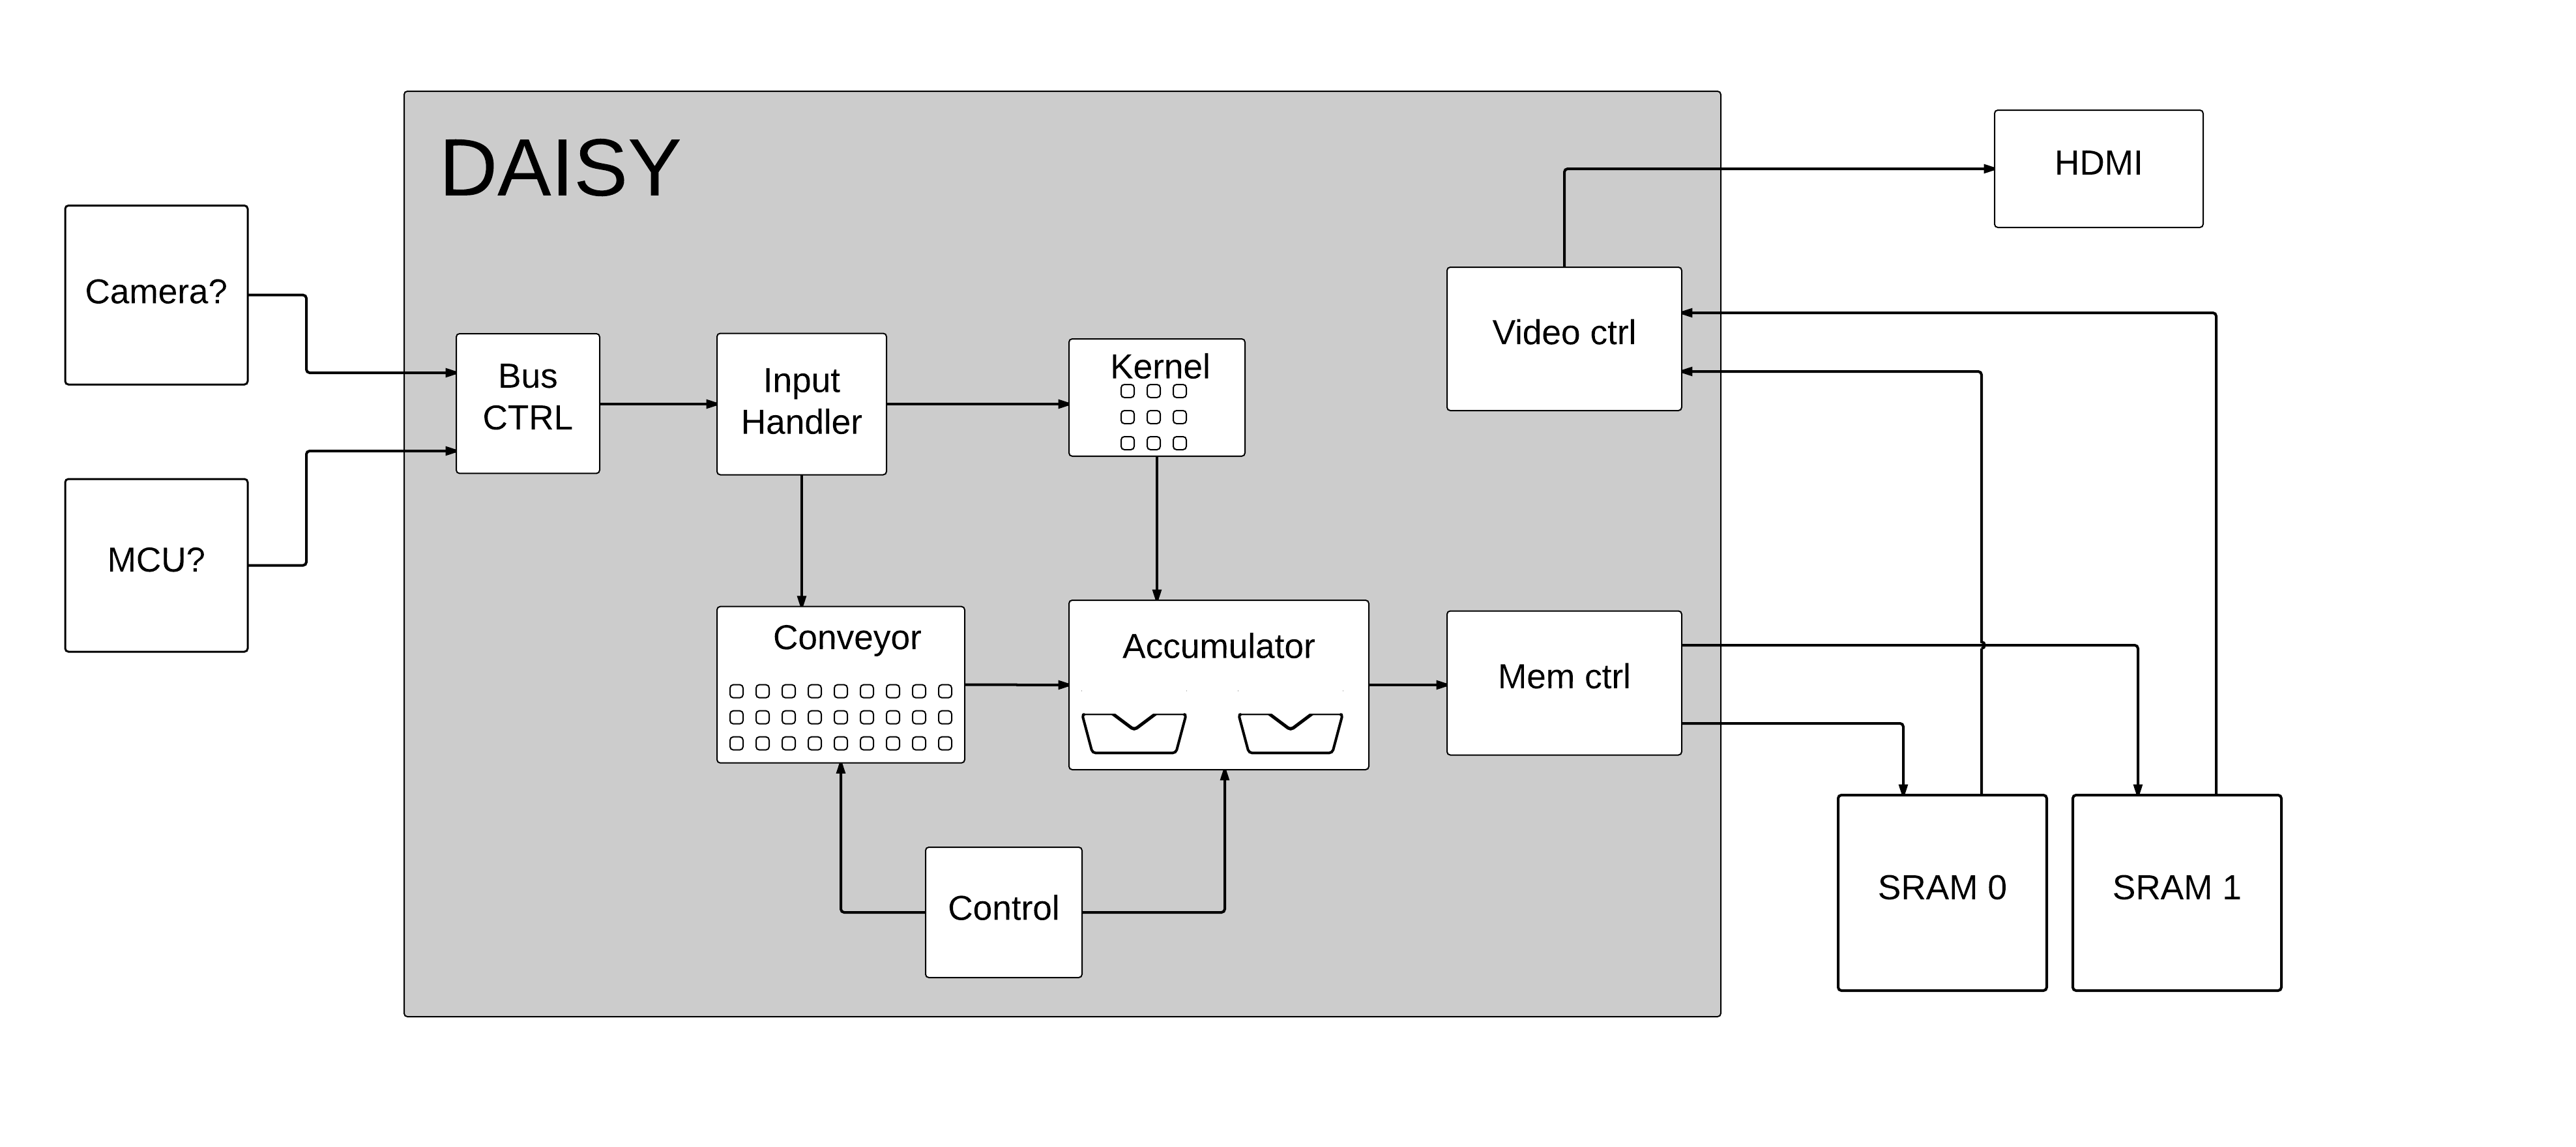
\includegraphics[width=\linewidth]{img/DataPath.png}
    \caption{The data path for our processor, named daisy after the way it daisy chains control}
    \label{fig:Convolution}
\end{figure}
In the figure we see this design principle reflected, no data ever flows backwards, only forwards. 
Breaking up the individual steps we get the typical flow of data.
\begin{enumerate}
  \item Data from the bus is read by the bus controller. This controller serves as a clock domain crossover and is responsible for delivering data to the input handler in a clock domain crossing FIFO queue.
  \item The input handler recieves data from the queue and does magic
  \item Pixel data is held in a special buffer with rows representing the current sweep window.
  \item The accumulator recieves kernel data from the kernel buffer and performs its mapping function on the kernel value and the pixel from the conveyor belt. 
When an accumulator has accumulated all its pixels it flushes its value, resetting the accumulator register and writing the old data to the memory control unit.
  \item Accumulated pixels are reassembled in the mem ctrl unit and written to one of the two SRAM banks, allowing us to double buffer. 
  \item After being buffered in SRAM pixel data is read by the video ctrl module which outputs video to an HDMI cable, ensuring crisp image quality served in a modern fashion.
\end{enumerate}

\subsection{Data in}
\begin{figure}[h!]
    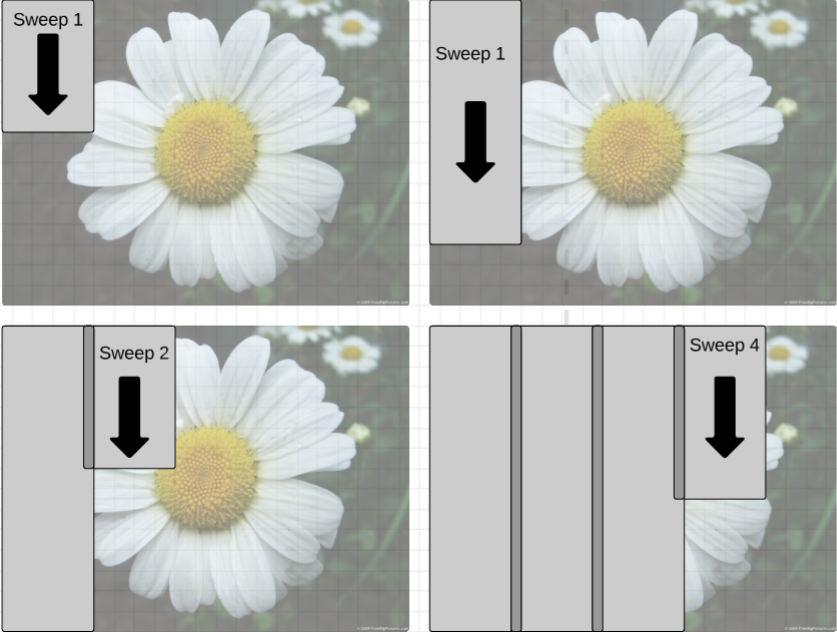
\includegraphics[width=\linewidth]{img/Sweeps.png}
    \caption{The sweep pattern used to collect data for convolution. The deep grey region indicates overlap, pixels which will be collected twice}
    \label{fig:Sweeps}
\end{figure}
Fig:Sweeps shows the pattern in which data is being fed into the processor.
A good analogy is how a squeegee (nal) is used to clean a window, by doing either horizontal or vertical sweeps.
In fig:SweepFrontier we show the area of the image we are currently working on.
Our workarea, or sweep window, is nine pixels wide and three deep, and for each row the convolutions that have the middle row as center pixels are calculated.
\begin{figure}[h!]
    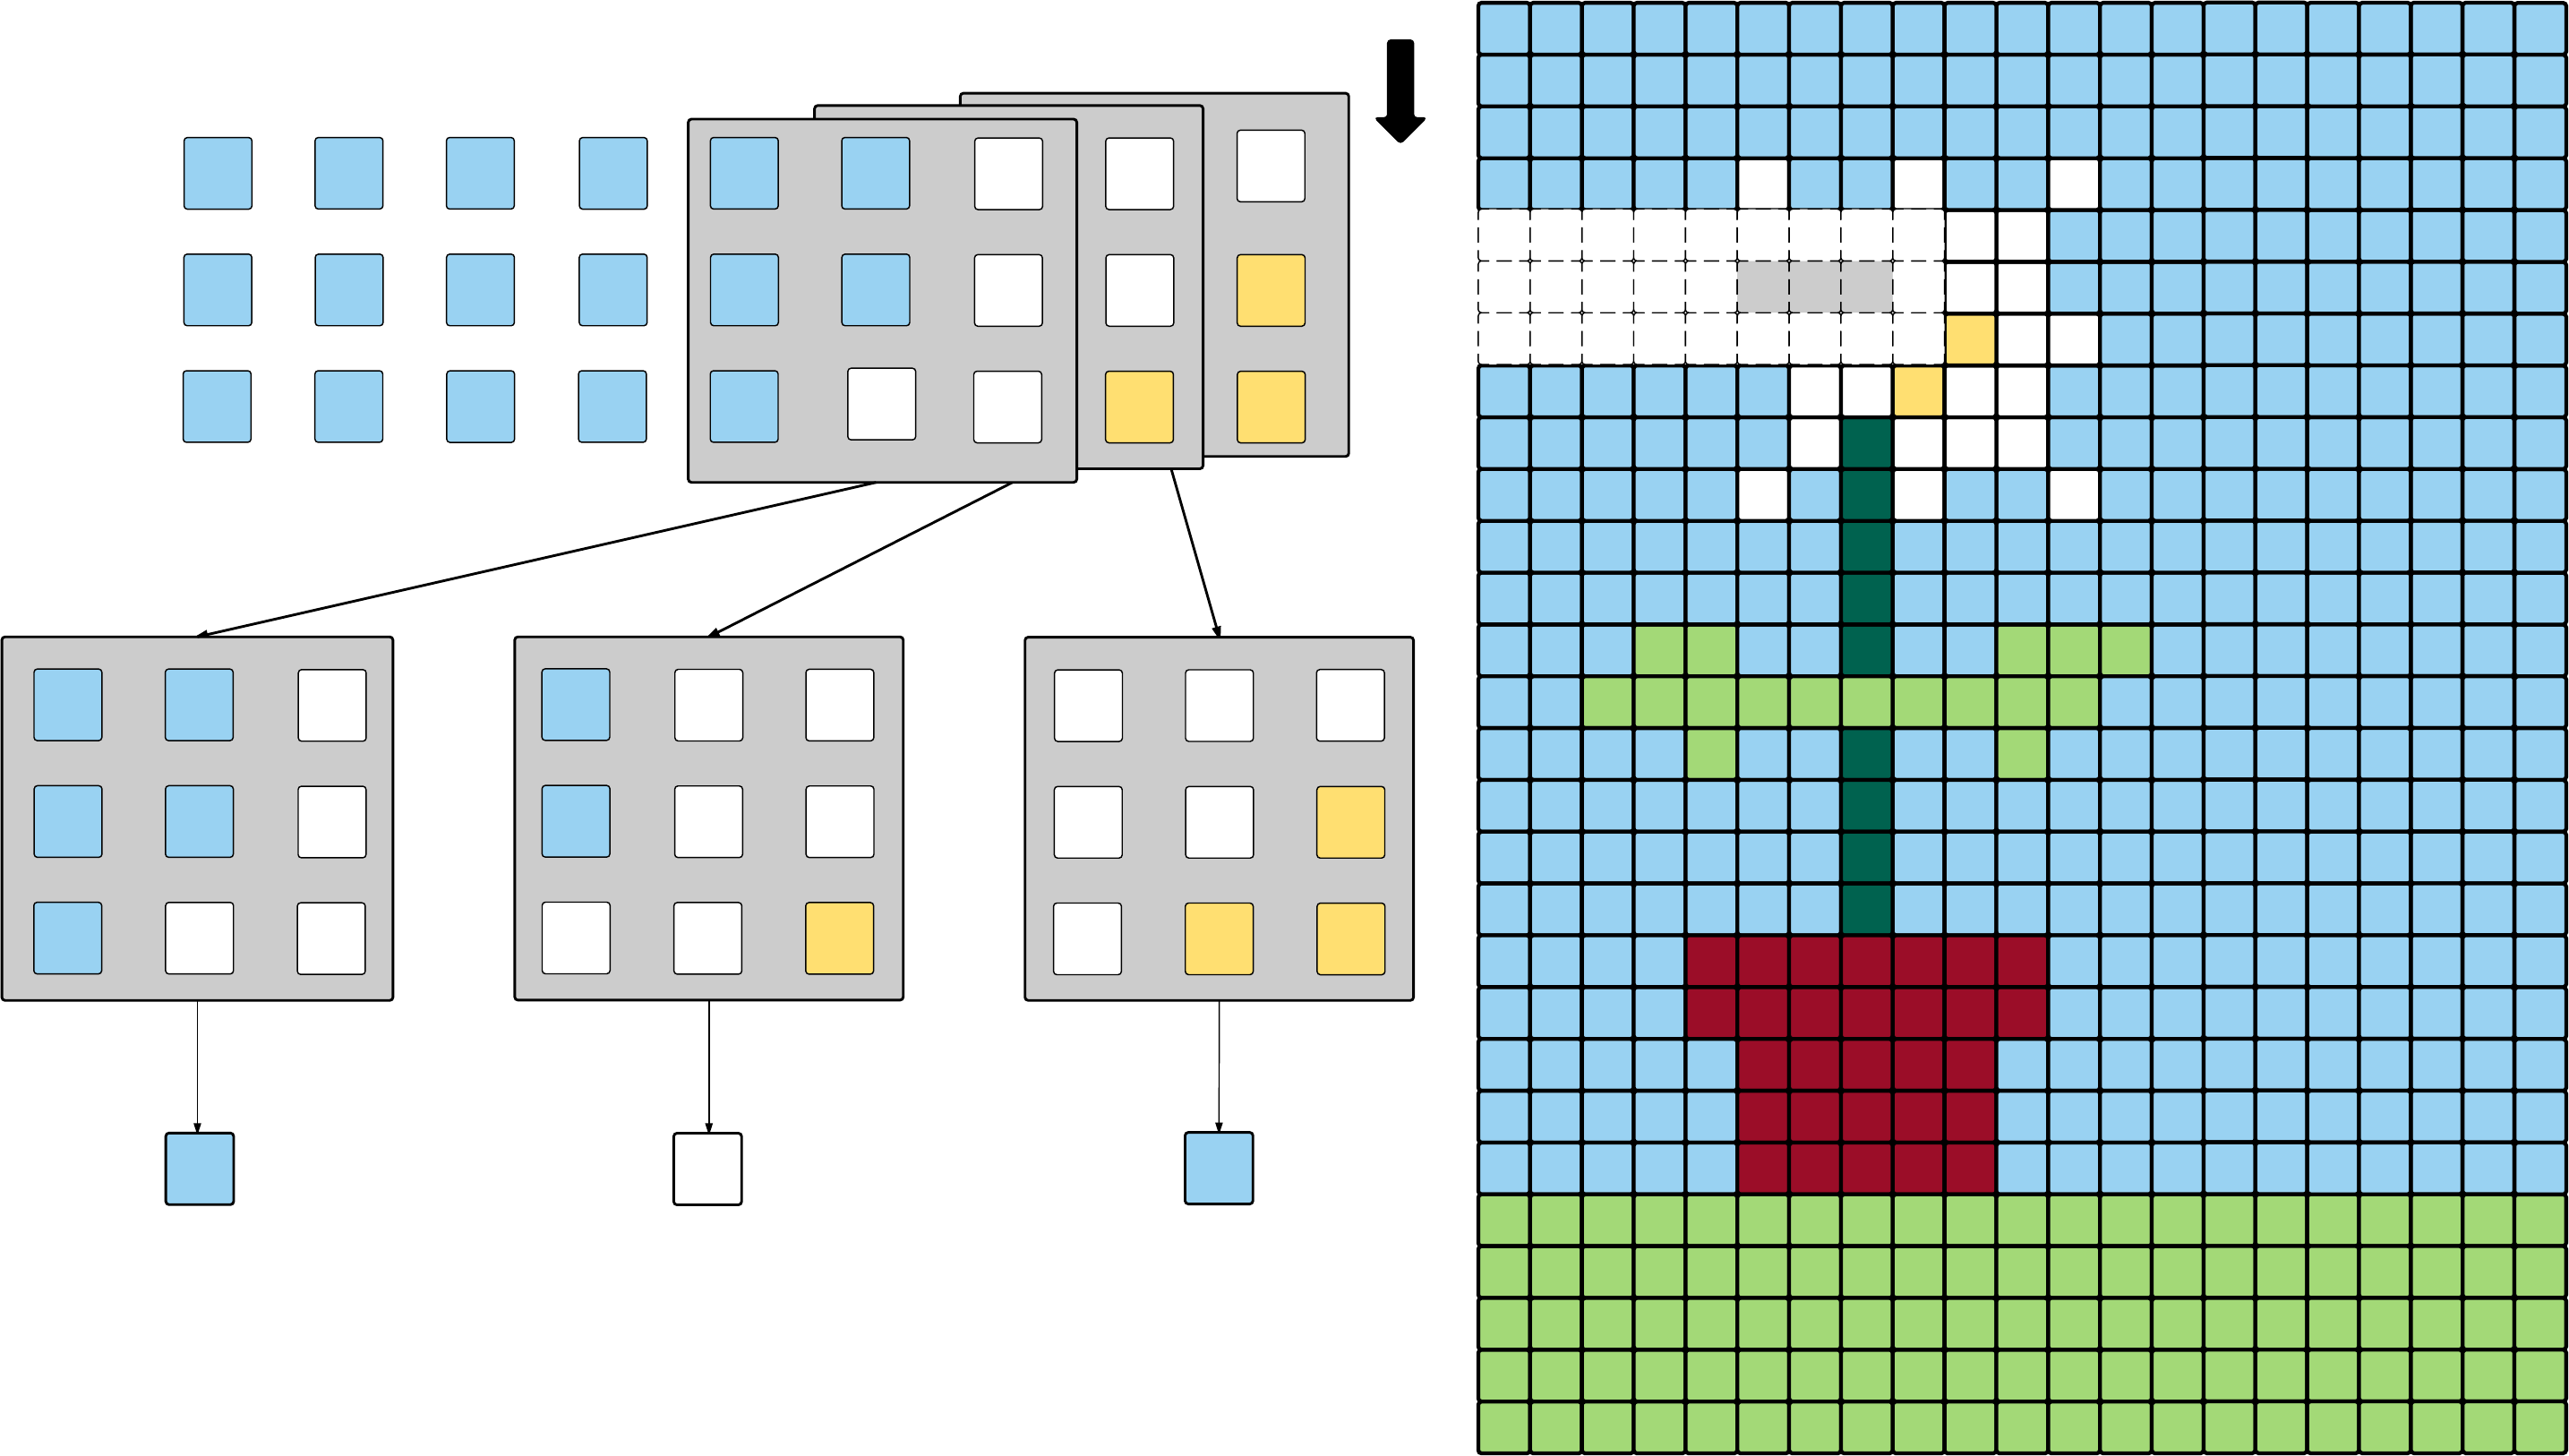
\includegraphics[width=\linewidth]{img/FeedPattern.png}
    \caption{The image three greyed out pixels in the source image represent the three pixels which the regions in grey boxes help calculate. The window is three pixels deep and nine pixels wide}
    \label{fig:SweepFrontier}
\end{figure}

\subsection{Convolver}
This section encompasses the four modules forming the heart of the convolution engine as depicted in fig:DaisyView. In the order they are covered, they are:
\begin{description}
    \item[the conveyor belt] \hfill\\ 
        A buffer responsible for maintaining the three rows of the sweep window and to feed the accumulator with three reads each cycle, one read from each row every cycle.
        The three rows must be read in such a way that each accumulator may collect the nine subpixels it needs per convolution by reading each conveyor output at the correct time.
    \item[the kernel buffer] \hfill\\
        The kernel buffer in the figure is an abstraction, in the implementation the kernel buffer resides much closer to the accumulators, but we separate it in our overview to show how each ALU in the accumulator reads kernel values.
    \item[the accumulator] \hfill\\
        The accumulator is being fed data over three wires, and by choosing which wires to read from ensures that each accumulator works on the correct subpixels.
    \item[the control unit] \hfill\\
        In order for the accumulators and pixel conveyor to be in sync a control unit sends control signals periodically, which are then propogated throughout the system.
\end{description}
Fig:DaisyView shows an overview of the four components in the heart of daisy. 
Lastly, 
\begin{figure}[h!]
    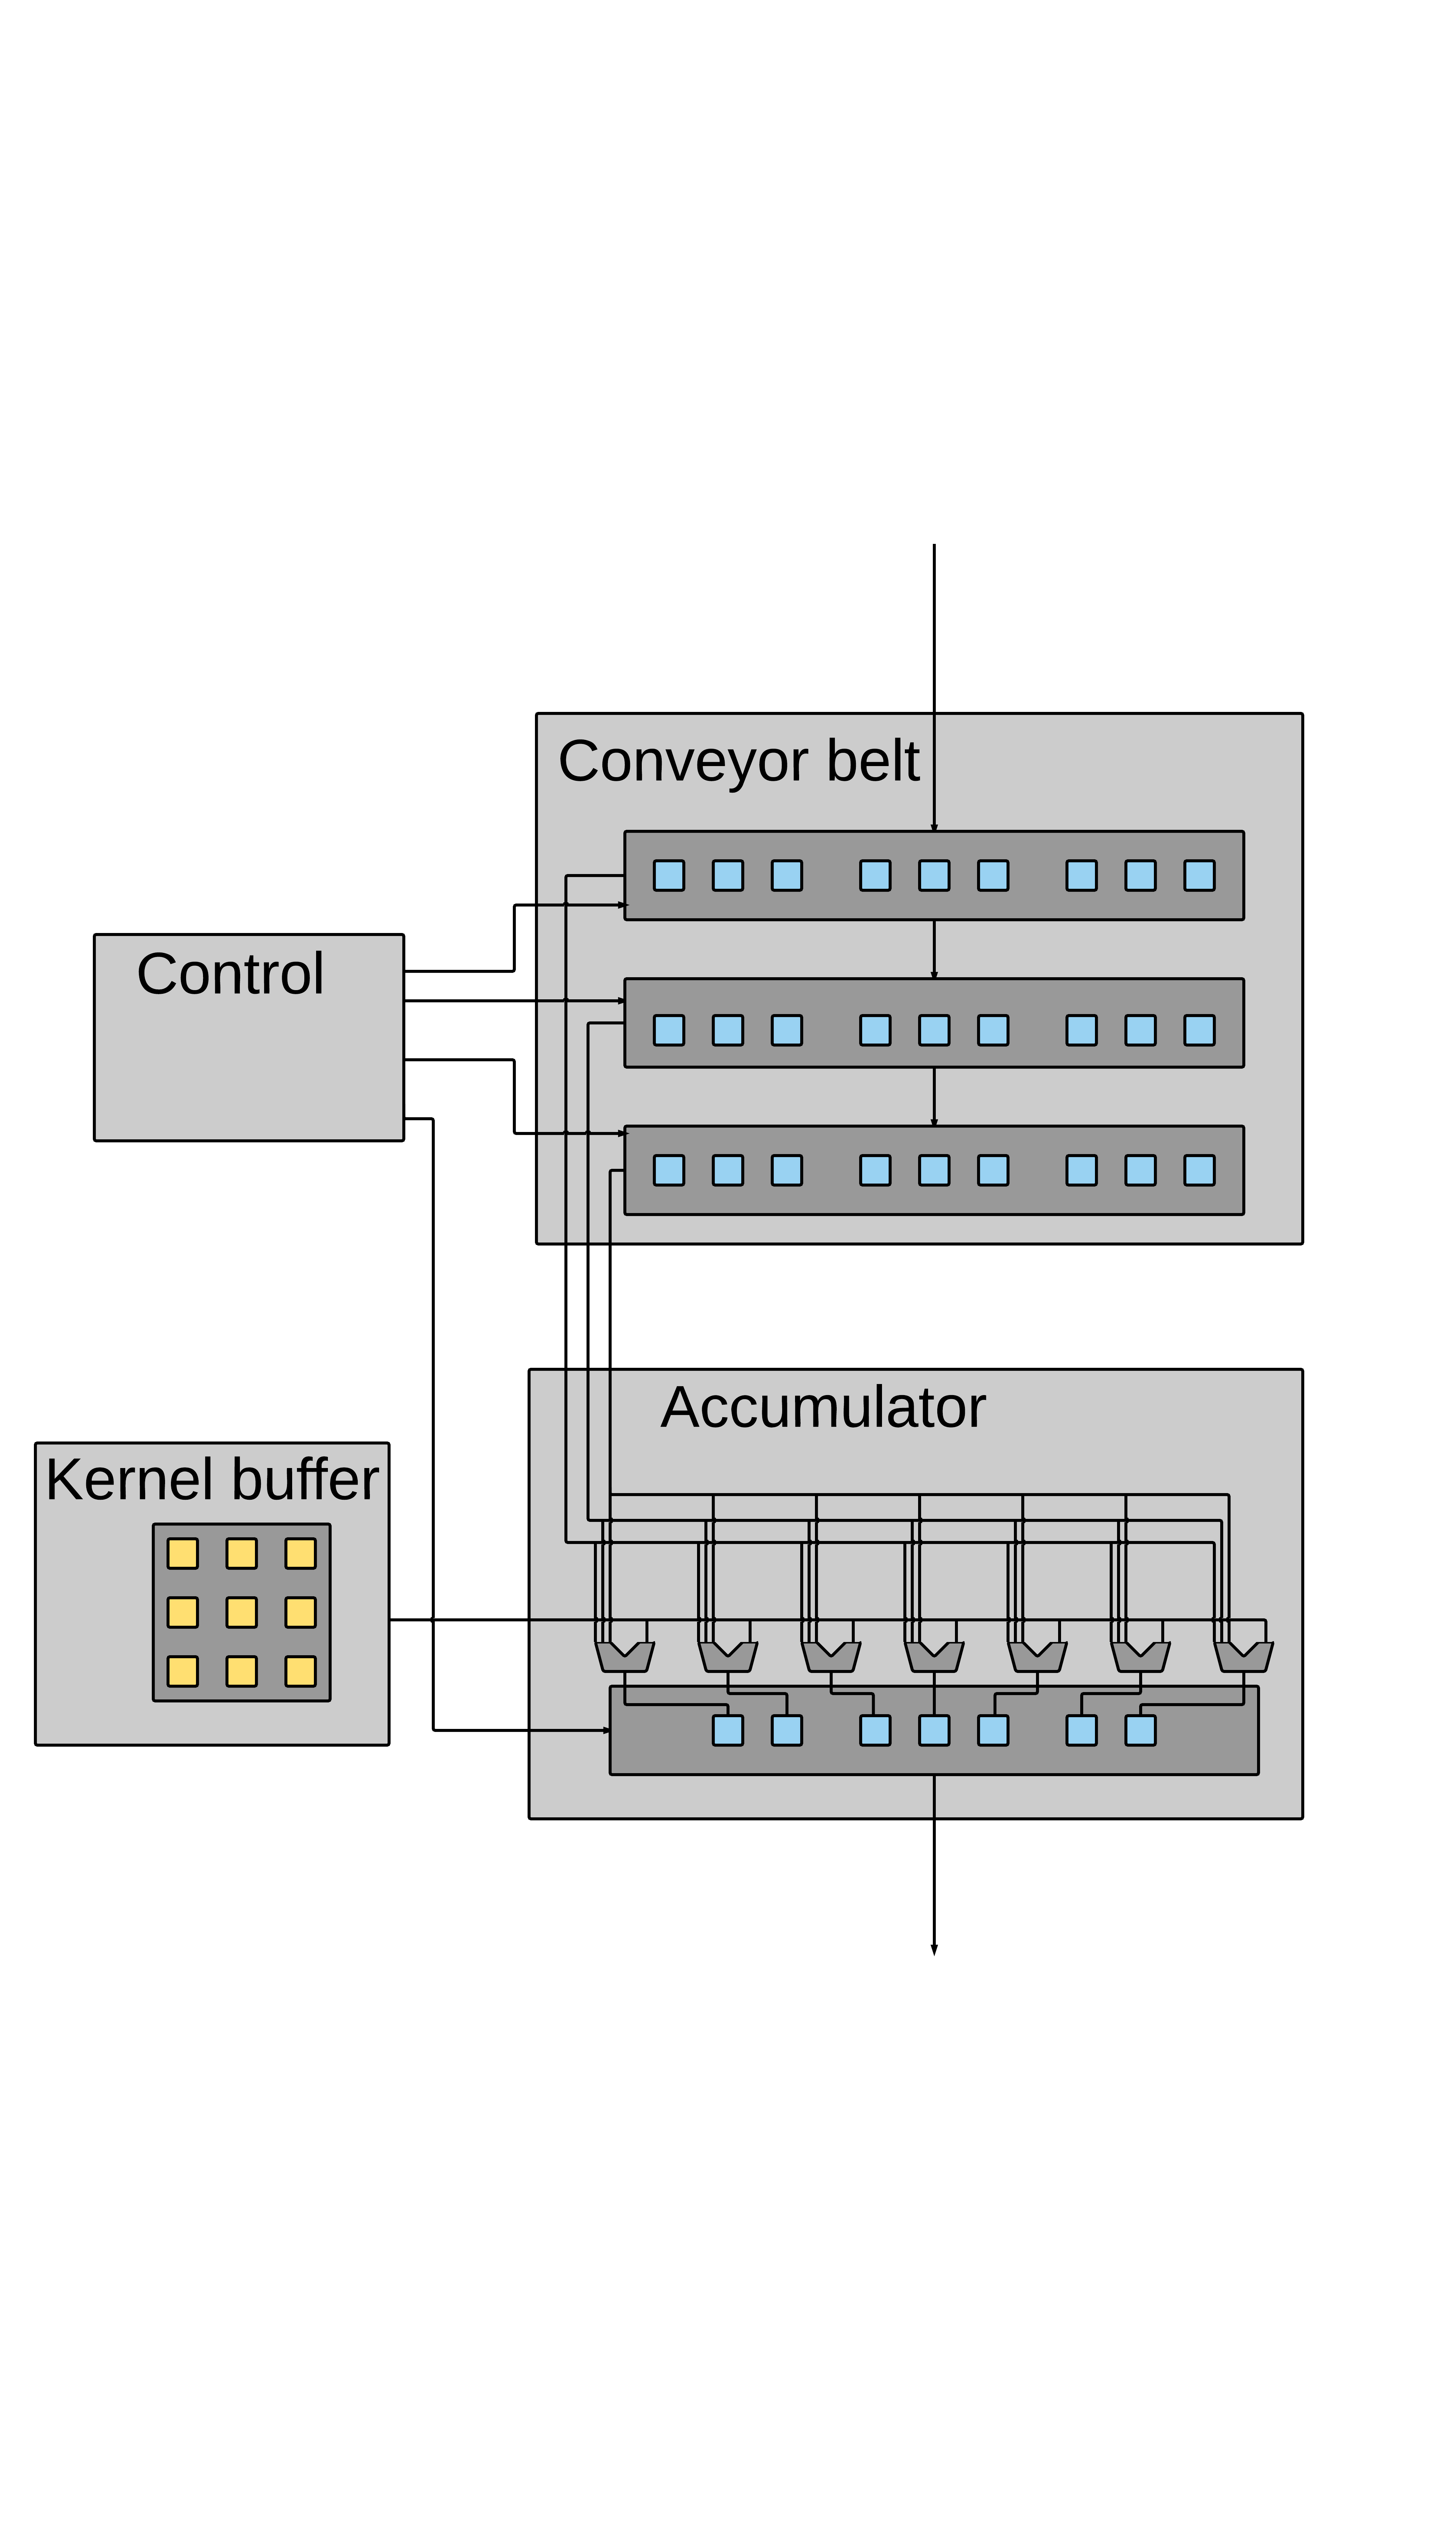
\includegraphics[width=\linewidth]{img/DaisyOverview.png}
    \caption{The four core units in the convolution process}
    \label{fig:DaisyView}
\end{figure}

\subsubsection{The accumulator}
Although the accumulator unit is the last unit in the datapath of daisy we will cover it first since it helps motivate the designs further up in the chain.
The accumulator actually consists of seven accumulators, hereby referred to as pixel accumulators. Each pixel accumulator corresponds to a pixel in the middle row.
The leftmost and the rightmost pixel in the middle row has no accumulator associated with it because it lacks three pixels necessary for a full convolution, necessetating the slight overlap in our feed pattern.
In fig:DaisyView the input from the conveyor is shown as three wires, one from each row.  
Each accumulator is responsible to read from the correct row at the correct time, such that it accumulates only the subpixels of the source pixel.\\ \\ \\
\\
\begin{tabular}{l*{16}{c}r}
    Time (cycle)        & $T_{0}$ & $T_{1}$ & $T_{2}$ & $T_{2}$ & $T_{4}$  & $T_{5}$ & $T_{6}$ & $T_{7}$ & $T_{8}$ & $T_{9}$ & $T_{10}$ & $T_{11}$ & $T_{12}$ & $T_{13}$ & $T_{14}$\\
\hline
Row 1                   & 4 & 5 & 6 & 7 & 8 & 9 & \cellcolor{gray75} 1 & \cellcolor{gray75} 2 & \cellcolor{gray75} 3 & 4 & 5 & 6 & 7 & 8 & 9 & \\
Row 2                   & 7 & 8 & 9 & \cellcolor{gray75} 1 & \cellcolor{gray75} 2 & \cellcolor{gray75} 3 & 4 & 5 & 6 & 7 & 8 & 9 & \cellcolor{gray75} 1 & \cellcolor{gray75} 2 & \cellcolor{gray75} 3 & \\
Row 3                   & \cellcolor{gray75} 1 & \cellcolor{gray75} 2 & \cellcolor{gray75} 3 & 4 & 5 & 6 & 7 & 8 & 9 & \cellcolor{gray75} 1 & \cellcolor{gray75} 2 & \cellcolor{gray75} 3 & 4 & 5 & 6 & \\
\end{tabular}\\ \\ \\
We will first focus on the leftmost accumulator starting at time T0 doing the following reads. 
It first reads three values from Row 3 which corresponds to its southwestern subpixel at $T_{0}$, its southern subpixel at $T_{1}$, and its southeastern subpixel at $T_{2}$, shown as the greyed out cells in row 3.
At time $T_{3}$ it starts reading from Row 2, reading its western, middle and eastern subpixels at respectively $T_{3}$, $T_{4}$, and $T_{5}$, shown as the greyed out cells in row 2.
Finally it reads its northwestern, northern and northwestern subpixel at time $T_{6}$ to $T_{8}$ from Row 1.
What about the second leftmost accumulator then? By following the exact same read pattern, but waiting one cycle allows it to read all its values in the same manner as the leftmost accumulator!
The second accumulator reads from Row 3 at time $T_{1}$, switches to Row 2 at $T_{4}$ and again to Row 1 from $T_{7}$ to $T_{9}$. 
In fact, every accumulator starts one cycle later than its left neighbour, meaning every accumulator has accumulated its necessary pixels at different times.
\\ \\
\begin{tabular}{l*{16}{c}r}
    Time (cycle)        & $T_{0}$ & $T_{1}$ & $T_{2}$ & $T_{2}$ & $T_{4}$  & $T_{5}$ & $T_{6}$ & $T_{7}$ & $T_{8}$ & $T_{9}$ & $T_{10}$ & $T_{11}$ & $T_{12}$ & $T_{13}$ & $T_{14}$\\
\hline
Row 1                   & \cellcolor{gray75} 4 & 5 & 6 & 7 & 8 & 9 & 1 & \cellcolor{gray75} 2 & \cellcolor{gray75} 3 & 4\cellcolor{gray75} & 5 & 6 & 7 & 8 & 9 & \\
Row 2                   & 7 & 8 & 9 & 1 & \cellcolor{gray75} 2 & \cellcolor{gray75} 3 & \cellcolor{gray75}4 & 5 & 6 & 7 & 8 & 9 & 1 & \cellcolor{gray75} 2 & \cellcolor{gray75} 3 & \\
Row 3                   & 1 & \cellcolor{gray75} 2 & \cellcolor{gray75} 3 & 4\cellcolor{gray75} & 5 & 6 & 7 & 8 & 9 & 1 & \cellcolor{gray75} 2 & \cellcolor{gray75} 3 & 4\cellcolor{gray75} & 5 & 6 & \\
\end{tabular}\\ \\ \\

\subsubsection{The conveyor belt}
As established last section, the job of the conveyor is to feed data from each of its rows to the accumulator.
In addition to serving data to the accumulator the conveyor must also feed new data to the belt and propogate that data downward which gives rise to its name.
In order to both propagate data downward and feed correct data to the accumulator as efficently as possible the conveyor will utilize the data from a read operation to both feed the accumulator and to transfer data laterally.
When a register is read, it is therefore the job of the register directly beneath it to read, conveying data downwards.
By studying the tables in the previous section we see that reads are done in a wave pattern, and consequentially so is the data conveying, which has a very powerful implication:
Since every accumulator and register will perform the same operation as its left neighbour offset by one cycle we can let each element be responsible for controlling the element to its right.
Rather than using a central control module we can instead simply daisy chain the control signals and interface only with the leftmost components, which also explains the name of the convolution core, Daisy.
An analogy to the read signals is a key. At time $T_{0}$ the control element gives the leftmost register the read key. 
The register does as it is told and reads its new value from the register above, and hands the key over to its neighbour. 
At $T_{1}$ the neighbour recieves the key, and reads from the register above it and sends the key further on.

TODO: Figure out a succint way to explain this part

\subsubsection{The controller}
We have established how control flows throughout the system, but we still need a module to give out keys to the leftmost accumulators and registers.
The controller is responsible for sending out the keys in the correct order and at the correct time.
Timing is everything, if we misalign read signals and write signals we may end up in a situation where a register fails to read when the register above it writes.
For example, if the controller sends each read signal one cycle too late each register will read when the register to the right side of the one directly above it, causing the data to be sheared as it moves laterally!
Other than issuing read and write keys to the registers, the controller also issues a flush key for the accumulators which tells accumulators to drive DATA\_OUT with its contents, and to reset.

\subsubsection{The kernel buffer}
In our schematic we present the kernel buffer as a separate submodule. 
However, having already introduced how instructions are daisy chained it makes sense to do the same with kernels since seven different kernel values are in use at all times.
Thus the kernel values are kept in a shift register queue living as close to the accumulators as possible, needing only two registers to hold the currently unused kernel values.
The responsibilities of the kernel unit is thus to collect the first data values into the kernel buffer chain and to buffer the two kernel values which are not currently in use.
